\section{案例研究:线性生成器}

在这一节中,我们将看到两个由线性函数构建的 PRG 的例子。这两个生成器都遵循 \ref{subsec:3-4-2} 小节中介绍的 Blum-Micali 范式。我们的第一个例子称为\emph{线性同构生成器},它是完全不安全的。我们之所以以它为例,是想举例说明攻击 PRG 时可能会出现的一些优美的数学构造。我们的第二个例子称为\emph{子集和生成器},如果我们假设经典子集和问题的某个特定版本是困难的,就可以证明它是一个安全的 PRG。

\subsection{一个密码分析的例子:线性同构生成器}

线性同构生成器(Linear congruential generators, LCG) 在统计模拟中被用于产生伪随机值。它们速度快,容易实现,并且被广泛部署。LCG 的变体也在 glibc、Microsoft Visual Basic 和 Java 运行时的早期版本中被用于引入随机性。虽然这些生成器可能足以用于模拟,但它们\emph{绝不}应该用在密码学应用中,因为它们作为 PRG 是不安全的。特别是它们是可预测的:给定 LCG 的几个连续输出,很容易计算出所有后续的输出。在本节中,我们通过展示一种预测算法来描述对 LCG 的攻击。

基本的线性同构生成器由四个公共系统参数指定:一个整数$q$,两个常数$a,b\in\{0,\dots,q-1\}$和一个正整数$w\leq q$。选取的常数$a$应与$q$互素。我们用$\mathcal{S}_q$和$\mathcal{R}$来表示集合:
\[
\mathcal{S}_q:=\{0,\dots,q-1\};\quad\quad
\mathcal{R}:=\{0,\dots,\lfloor(q-1)/w\rfloor\}
\]
这里的$\lfloor\cdot\rfloor$是向下取整函数:对于一个实数$x$,$\lfloor x\rfloor$是小于或等于$x$的最大整数。现在,以$s\in\mathcal{S}_q$为种子的生成器$G_\mathrm{lcg}:\mathcal{S}_q\to\mathcal{R}\times\mathcal{S}_q$的定义如下:
\[
G_\mathrm{lcg}(s):=\big(
\lfloor s/w \rfloor,\;
as+b\;\mathrm{mod}\;q
\big)
\]
当$w$是$2$的幂,比如$w=2^t$时,$\lfloor s/w \rfloor$的计算其实就是简单地抹除$s$的$t$个最小有效位。因此,$G_\mathrm{lcg}(s)$的左边就是抹去$s$的$t$个最小有效位的结果。

生成器$G_\mathrm{lcg}(s)$显然是不安全的,因为只要给定$s':=as+b\;\mathrm{mod}\;q$,我们就可以直接重建$s$,然后将$\lfloor s/w \rfloor$从随机值中区分出来。然而,考虑下面的一种 Blum-Micali 构造的变体,其中,最终的 $\mathcal{S}_q$ 中的值不被输出:

\vspace*{5pt}

\hspace*{5pt} $G_\mathrm{lcg}^{(n)}(s):=$
\hspace*{20pt} $s_0\leftarrow s$\\
\hspace*{100pt} 对于 $j\leftarrow0$ 到 $L-1$:\\
\hspace*{100pt} \quad\quad\quad$r_i\leftarrow\lfloor s_{i-1}/w \rfloor,\quad s_i\leftarrow as_{i-1}+b\;\mathrm{mod}\;q$\\
\hspace*{100pt} 输出 $(r_0,\dots,r_n)$。

\vspace*{5pt}
我们将每一次循环称为LCG的一次迭代,并称每一个$r_1,\dots,r_n$为一次迭代的输出。

不同的实现会使用不同的系统参数$q$,$a$,$b$和$w$。例如,Java 8 中的 \texttt{Math.random} 函数使用 $q=2^{48}$,$w=2^{22}$ 以及十六进制常数$a=\texttt{0x5DEECE66D}$,$b=\texttt{0x0B}$。因此,LCG的每次迭代都会输出$48$比特的状态$s_i$的前$48-22=26$比特。

这个Java 8生成器所使用的参数对于安全应用来说显然太小了,因为生成器的第一次迭代输出就会揭示$s$中除了$22$比特之外的所有其他比特。攻击者可以通过穷举搜索轻易地恢复未知的这$22$比特:对于这$22$比特的每一个可能的值,它都生成一个候选种子$\hat s$。它可以从$\hat s$出发计算若干后续的输出,并将其与从实际的生成器中观察到的后续比特进行对比,以此来测试$\hat s$是否是正确的种子。只要遍历所有$2^{22}$个候选种子(约400万个),攻击者就能最终找到正确的种子$s$,然后就可以预测胜生成器的所有后续输出。这种攻击在现代处理器上的运行时间只有不到一秒。

就算LCG的参数大到足以抵抗穷举搜索,比如说$q=2^{512}$,生成器$G_\mathrm{lcg}$也是不安全的。就算你可以从各种软件库中找到它,也永远不要把它用在安全应用中。已知的针对 LCG 的攻击表明,即使生成器每次迭代只输出几个比特,我们仍有可能基于几个连续的输出预测整个序列。让我们看看这种攻击的一个优雅的版本。

\begin{snote}[密码分析。]
假设$q$很大(例如$q=2^{512}$),LCG $G_\mathrm{lcg}$ 每次迭代都会输出状态$s$中大约一半的比特,就像Java 8 中的 \texttt{Math.random}生成器一样。鉴于种子$s$的大小,对其进行穷举式搜索是不可能的。然而,我们下面展示,如何用仅仅两个连续迭代的输出来快速地预测生成器。

更确切地说,假设对于某个固定的$c>0$,例如$c=32$,有$w<\sqrt{q}/c$。这意味着在每次迭代中,生成器所输出的比特数都只略长于当前内部状态的比特数的一半。假设攻击者得到了生成器的连续两个输出$r_i,r_{i+1}\in\mathcal{R}$。我们下面展示它预测剩余序列的方法。对于某个未知的$s_i\in\mathcal{S}_q$,攻击者知道:
\[
r_i=\lfloor s_i/w\rfloor,\quad\quad
r_{i+1}=\lfloor s_{i+1}/w\rfloor=\lfloor(as_i+b\;\mathrm{mod}\;q)/w\rfloor
\]
我们有:
\[
r_i\cdot w+e_0=s_i,\quad\quad
r_{i+1}\cdot w+e_1=(as_i+b\;\mathrm{mod}\;q)
\]
其中,$e_0$和$e_1$是$s_i$和$s_{i+1}$除以$w$后的余数;特别地,我们有$0\leq e_0,e_1<w<\sqrt{q}/c$。$e_0$和$e_1$小于$\sqrt{q}$这一事实是攻击能够成功的一个重要因素。接下来,我们用$s$代换$s_i$,并引入一个整数变量$x$来消除$\mathrm{mod}\;q$,得到:
\[
r_i\cdot w+e_0=s,\quad\quad
r_{i+1}\cdot w+e_1=as+b+qx
\]
攻击者不知道$x$,$s$,$e_0$和$e_1$的值,但它知道$r_i$,$r_{i+1}$,$w$,$a$和$b$。最后,重新排列各项,把涉及$x$和$s$的项放到左边,得到:
\begin{equation}\label{eq:3-12}
s=r_i\cdot w+e_0,\quad\quad
as+qx=r_{i+1}w-b+e_1
\end{equation}
我们可以将式 \ref{eq:3-12} 重写为向量形式:
\begin{equation}
s\cdot
\begin{pmatrix}
1\\a
\end{pmatrix}
+x\cdot
\begin{pmatrix}
0\\q
\end{pmatrix}
=\boldsymbol{g}+\boldsymbol{e}
\quad\quad\text{where}\quad\quad
\boldsymbol{g}:=
\begin{pmatrix}
r_iw\\r_{i+1}w-b
\end{pmatrix}
,\;\;
\boldsymbol{e}:=
\begin{pmatrix}
e_0\\e_1
\end{pmatrix}
\end{equation}
令$\boldsymbol{u}\in\mathbb{Z}^2$表示未知向量$\boldsymbol{u}:=\boldsymbol{g}+\boldsymbol{e}=s\cdot(1,a)^\mathrm{T}+x\cdot(0,q)^\mathrm{T}$。如果攻击者能够找到$\boldsymbol{u}$,他就可以通过线性代数轻松地从$\boldsymbol{u}$中恢复$s$和$x$。利用$s$,他就可以预测PRG的其余输出。因此,想要破解生成器,只需要找到这样的向量$\boldsymbol{u}$即可。攻击者知道向量$\boldsymbol{g}\in\mathbb{Z}^2$,此外,他也知道$\boldsymbol{e}$很短,即$\lVert\boldsymbol{e}\rVert_\infty$最大为$\sqrt{q}/c$。因此,他知道$\boldsymbol{u}$是``接近" $\boldsymbol{g}$的。

我们下面展示如何由$\boldsymbol{g}$找到$\boldsymbol{u}$。考虑向量$(1,a)^\mathrm{T}$和$(0,q)^\mathrm{T}$的所有整系数线性组合所构成的集合。我们用$\mathcal{L}_a$表示这个集合,它是$\mathbb{Z}^2$的一个子集,包含像$(1,a)^\mathrm{T}$,$(2,2a)^\mathrm{T}$,$(3,3a-2q)^\mathrm{T}$这样的向量。图 \ref{fig:3-9} 展示了集合 $\mathcal{L}_a$,图中的实心点是向量$(1,a)^\mathrm{T}$和$(0,q)^\mathrm{T}$的整系数线性组合。我们称集合$\mathcal{L}_a$为由向量$(1,a)^\mathrm{T}$和$(0,q)^\mathrm{T}$所生成的二维\textbf{网格(lattice)}。

\begin{figure}
  \centering
  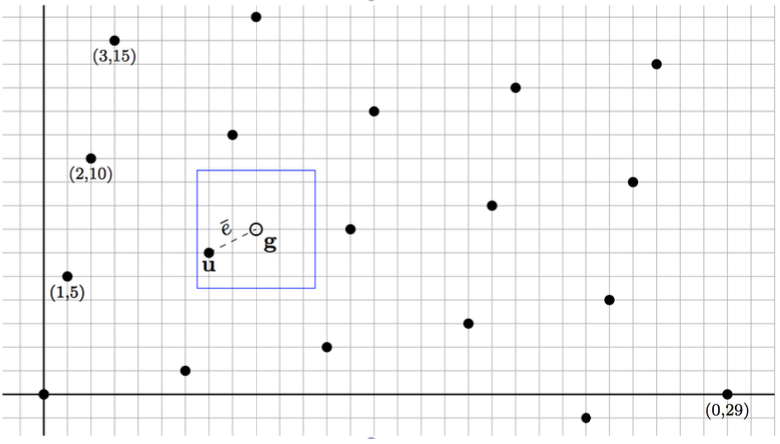
\includegraphics[width=0.6\linewidth]{figures/chapter3/fig9.png}
  \caption{与攻击LCG相关的二维网格。这里的网格是由向量$(1,5)^\mathrm{T}$和$(0,29)^\mathrm{T}$生成的。攻击者持有向量$\boldsymbol{g}=(9,7)^\mathrm{T}$,并希望找到最接近的网格向量$\boldsymbol{u}$。在这本图中确实只有一个``接近" $\boldsymbol{g}$ 的网格向量。}
  \label{fig:3-9}
\end{figure}

现在,攻击者有一个向量$\boldsymbol{g}\in\mathbb{Z}^2$,并且知道他的目标向量$\boldsymbol{u}\in\mathcal{L}_a$接近$\boldsymbol{g}$。如果他能在$\mathcal{L}_a$中找到与$\boldsymbol{g}$最接近的向量,那么这个向量很有可能就是所需的向量$\boldsymbol{u}$。下面的定理将表明,对于大多数的$a\in\mathcal{S}_q$来说,情况确实如此。
\end{snote}

\begin{lemma}\label{lemma:3-7}
对于$\mathcal{S}_q$中的至少$(1-16/c^2)\cdot q$个$a$,网格$\mathcal{L}_a\subseteq\mathbb{Z}^2$有如下性质:对于每个$\boldsymbol{g}\in\mathbb{Z}^2$,最多只有一个向量$\boldsymbol{u}\in\mathcal{L}_a$ 使得$\lVert\boldsymbol{g}-\boldsymbol{u}\rVert_\infty < \sqrt{q}/c$。
\end{lemma}

在引理 \ref{lemma:3-7} 中取$c=32$(因此$w=\sqrt{q}/30$),那么对于$98\%$的$a\in\mathcal{S}_q$来说,$\mathcal{L}_a$中离$\boldsymbol{g}$最近的向量就恰好是所需的向量$\boldsymbol{u}$。在证明该定理之前,我们首先完成对攻击的描述。

剩下的工作就是有效地找到$\mathcal{L}_a$中离$\boldsymbol{g}$最近的向量。这个问题是一个一般问题的特例,它叫做\textbf{最近向量问题(closest vector problem)}:给定一个网格$\mathcal{L}$和一个向量$\boldsymbol{g}$,找到$\mathcal{L}$中离$\boldsymbol{g}$最近的向量。有了这个算法,攻击者就可以根据生成器的两个输出$r_i$和$r_{i+1}$恢复 LCG 的内部状态$s_i$,并预测剩余的序列。这种攻击对$98\%$的$a\in\mathcal{S}_q$都有效。

完整起见,我们注意到,还有$2\%$的$a\in\mathcal{S}_q$所发起的攻击会失败,比如$a=1$和$a=2$。对于这些$a$,在$\mathcal{L}_a$中可能有多个接近给定的$\boldsymbol{g}$的网格向量。我们把设计一个对于 $\mathcal{S}_q$ 中那些不适用于引理 \ref{lemma:3-7} 的 $a$ 有效的攻击作为一个有趣的练习。最后,我们以对引理 \ref{lemma:3-7} 的证明结束本节。

\begin{proof}[引理 \ref{lemma:3-7} 的证明]
令$\boldsymbol{g}\in\mathbb{Z}^2$,假设$\mathcal{L}_a$中存在两个接近$\boldsymbol{g}$的向量$\boldsymbol{u}_0$和$\boldsymbol{u}_1$,即$\lVert\boldsymbol{u}_i-\boldsymbol{g}\rVert_\infty<\sqrt{q}/c$对于$i=0,1$成立。那么$\boldsymbol{u}_0$和$\boldsymbol{u}_1$一定是相互接近的。事实上,根据三角不等式,我们有:
\[
\lVert\boldsymbol{u}_0-\boldsymbol{u}_1\rVert_\infty\leq\lVert\boldsymbol{u}_0-\boldsymbol{g}\rVert_\infty+\lVert\boldsymbol{g}-\boldsymbol{u}_1\rVert_\infty\leq2\sqrt{q}/c
\]
由于任何网格在加法下都是封闭的,因此我们可以看出$\boldsymbol{u}:=\boldsymbol{u}_0-\boldsymbol{u}_1$是网格$\mathcal{L}_a$中的一个向量,并且我们可以得出结论:$\mathcal{L}_a$中一定包含一个``短"向量,即一个范数最大为$B:= 2\sqrt{q}/c$的非零向量。因此,我们对使得$\mathcal{L}_a$包含这样一个短向量的``坏的" $a$ 的数量进行约束。

我们首先考虑$q$是素数的情况。我们声称,每个短向量最多包含在一个网格$\mathcal{L}_a$中,因此坏的$a$的数量最多就是短向量的数量。假设$\boldsymbol{t}=(s,y)^\mathrm{T}\in\mathbb{Z}^2$是某个非零向量,满足$\lVert\boldsymbol{t}\rVert_\infty\leq B$。假设对于某个$a\in\mathcal{S}_q$有$\boldsymbol{t}\in\mathcal{L}_a$,那么存在整数$s_a$和$x_a$使得$s_a\cdot(1,a)^\mathrm{T}+x_a\cdot(0,q)^\mathrm{T}=\boldsymbol{t}=(s,y)^\mathrm{T}$。由此,我们得到$s=s_a$和$y=as\;\mathrm{mod}\;q$。此外,我们有$s\neq0$,因为如果不是这样,就有$\boldsymbol{t}=\boldsymbol{0}$。因为$y=as\;\mathrm{mod}\;q$,$s\neq0$,所以$a$的值是唯一确定的,即$a=ys^{-1}\;\mathrm{mod}\;q$。因此,当$q$是素数时,每个非零的短向量$\boldsymbol{t}$都最多只包含在一个$a\in\mathcal{S}_q$的网格中。进而可知,坏的$a$的数量最多就是短向量的数量,也就是$(2B)^2=16q/c^2$。

当$q$不是素数时,对坏的$a$的数量的约束同样成立。为了说明原因,考虑一个特定的非零$s\in\mathcal{S}_q$,令$d=\gcd(s, q)$。如上所述,只有当有一个$a\in\mathcal{S}_q$满足$as\equiv y\;(\mathrm{mod}\;q)$时,向量$\boldsymbol{t}=(s,y)^\mathrm{T}$才包含在某个网格$\mathcal{L}_a$中。这意味着$y$必须是$d$的倍数,所以我们只需要考虑$y$的$2B/d$个可能取值。对于每个这样的$y$,向量$\boldsymbol{t}=(s,y)^\mathrm{T}$最多包含在$d$个网格中。由于$s$有$2B$个可能取值,这表明坏的$a$的数量以$d\cdot 2B/d \cdot 2B=(2B)^2$为界,这与$q$是素数的情况相同。

总之,$\mathcal{S}_q$中最多有$16q/c^2$个坏的$a$。因此,对于$\mathcal{S}_q$中的$(1-16/c^2)\cdot q$个$a$值,网格$\mathcal{L}_a$中不包含非零短向量,故而该引理得证。
\end{proof}

\subsection{子集和生成器}

接下来我们展示如何基于简单的线性运算构建一个伪随机生成器。假设经典\emph{子集和问题(subset sum problem)}的某个随机版本是困难的,那么这个生成器是安全的。

\begin{snote}[模子集问题。]
令$q$是一个正整数,令$\mathcal{S}_q:=\{0,\dots,q-1\}$。在$\mathcal{S}_q$中选择$n$个整数$\boldsymbol{a}:=(a_0,\dots,a_{n-1})$,并定义子集和函数 $f_{\boldsymbol{a}}:\{0,1\}^n\to\mathcal{S}_q$为:
\[
f_{\boldsymbol{a}}(\boldsymbol{s}):=\sum_{i:s_i=1}a_i\;\mathrm{mod}\;q
\]
比如说 $f_{\boldsymbol{a}}(101101)=a_0+a_1+a_2+a_4\;\mathrm{mod}\;q$。现在,对于一个目标整数$t\in\mathcal{S}_q$,模子集问题的定义如下:
\begin{quote}
给定$(q,\boldsymbol{a},t)$作为输入,如果存在一个向量$\boldsymbol{s}\in\{0,1\}^n$使得$f_{\boldsymbol{a}}(\boldsymbol{s})=t$,则将其输出。
\end{quote}
换句话说,该问题是,如果函数$f_{\boldsymbol{a}}(\cdot)$存在反函数,就通过寻找$t$的原像的方式来求得该反函数。模子集问题目前被认为是 NP 困难的。
\end{snote}

\begin{snote}[子集和与PRG。]
子集问题自然而然地给出了以下的PRG:在设置时选择一个固定整数$q$,并从$\mathcal{S}_q$中随机选择$n$个整数$\vec{a}:=(a_0,\dots,a_{n-1})$。PRG $G_{q,\vec{a}}$将一个种子$\boldsymbol{s}\in\{0,1\}^n$作为输入,并输出一个$\mathcal{S}_q$上的伪随机值。其定义为:
\[
G_{q,\vec{a}}(\boldsymbol{s}):=\sum_{i=1}^na_i\cdot s_i\;\mathrm{mod}\;q
\]
该 PRG 将一个$n$比特的种子拉伸为一个$\log_2q$比特的输出。选择$n$和$q$使得$2n=\log_2q$,我们就可以得到一个 PRG,其输出长度是输入长度的两倍。我们可以将其插入 Blum-Micali 构造中以进一步扩大输出。

虽然这个 PRG 比 \ref{sec:3-6} 节中的 ChaCha20 等自定义构造要慢得多,但每一位输出所对应的工作都只是$\mathcal{S}_q$上的一个模加法,这可能适合一些对时间不敏感的应用。

Impagliazzo和Naor表明,攻击基于$G_{q,\vec{a}}$的PRG的难度与解决模子集和问题的某个随机化变体一样。虽然已经有很多工作试图解决模子集问题,但对于较大的$n$,比如$n>1000$,当$2n=\log_2q$时,该问题似乎仍然是很难的,这就意味着$G_{q,\vec{a}}$作为 PRG 是安全的。
\end{snote}

\begin{snote}[变体。]
Fischer和Stern等人提出子集和生成器的一个变体:
\[
G_{q,\vec{a}}(\boldsymbol{s}):=A\cdot\boldsymbol{s}\;\mathrm{mod}\;q
\]
其中,$q$是一个小素数,$A$是一个$\mathcal{S}_q^{n\times m}$上的随机矩阵,$n<m$,并且种子$\boldsymbol{s}$均匀分布在$\{0,1\}^m$上。该生成器将$m$比特的种子映射为$n\log_2q$比特的输出。我们将在第\ref{chap:16}章进一步讨论这个生成器。
\end{snote}















